\subsection{Host Galaxy Properties} \label{subsec: Host Galaxy Properties}
In section \ref{subsec: Progenitor Channels} it's clear that the environment of the SNe plays a factor in the shape of the light curve observed from an SN. Thus the properties of the host galaxies of SNe have been studied to determine the correlations between those properties and the locations of where SNe happen. \textcite{toy_reduction_2025} uses a sample of 1533 SNe Ia from the 'five-year' sample from the DES SN program. \textcite{toy_reduction_2025} using the Directional Light Radius method (DLR) to associate SNe Ia with a host galaxy and find that there is no step-like change in the Hubble residuals average across a normalised DLR, \(d_{DLR}\), of 1. But when splitting the sample to 'inner regions' where \(d_{DLR} < 1\) the Hubble residuals have a step in the averages of \(0.100 \pm 0.014\) mag when split across the host galaxies with a stellar mass of 10. But in the outer regions (\(d_{DLR}>1\)) \textcite{toy_reduction_2025} finds that the step in the Hubble residuals when split by host's with stellar masses of 10 is \(0.036\pm0.018\). \textcite{toy_reduction_2025} makes the conclusion that SNe Ia in the outer regions are less affected by the global host galaxy properties, although \textcite{toy_reduction_2025} notes that the different mechanics that produce this result is still unknown.

\begin{figure}[htbp]
     \centering
     % Top Image
     \begin{subfigure}[b]{0.6\textwidth}
         \centering
         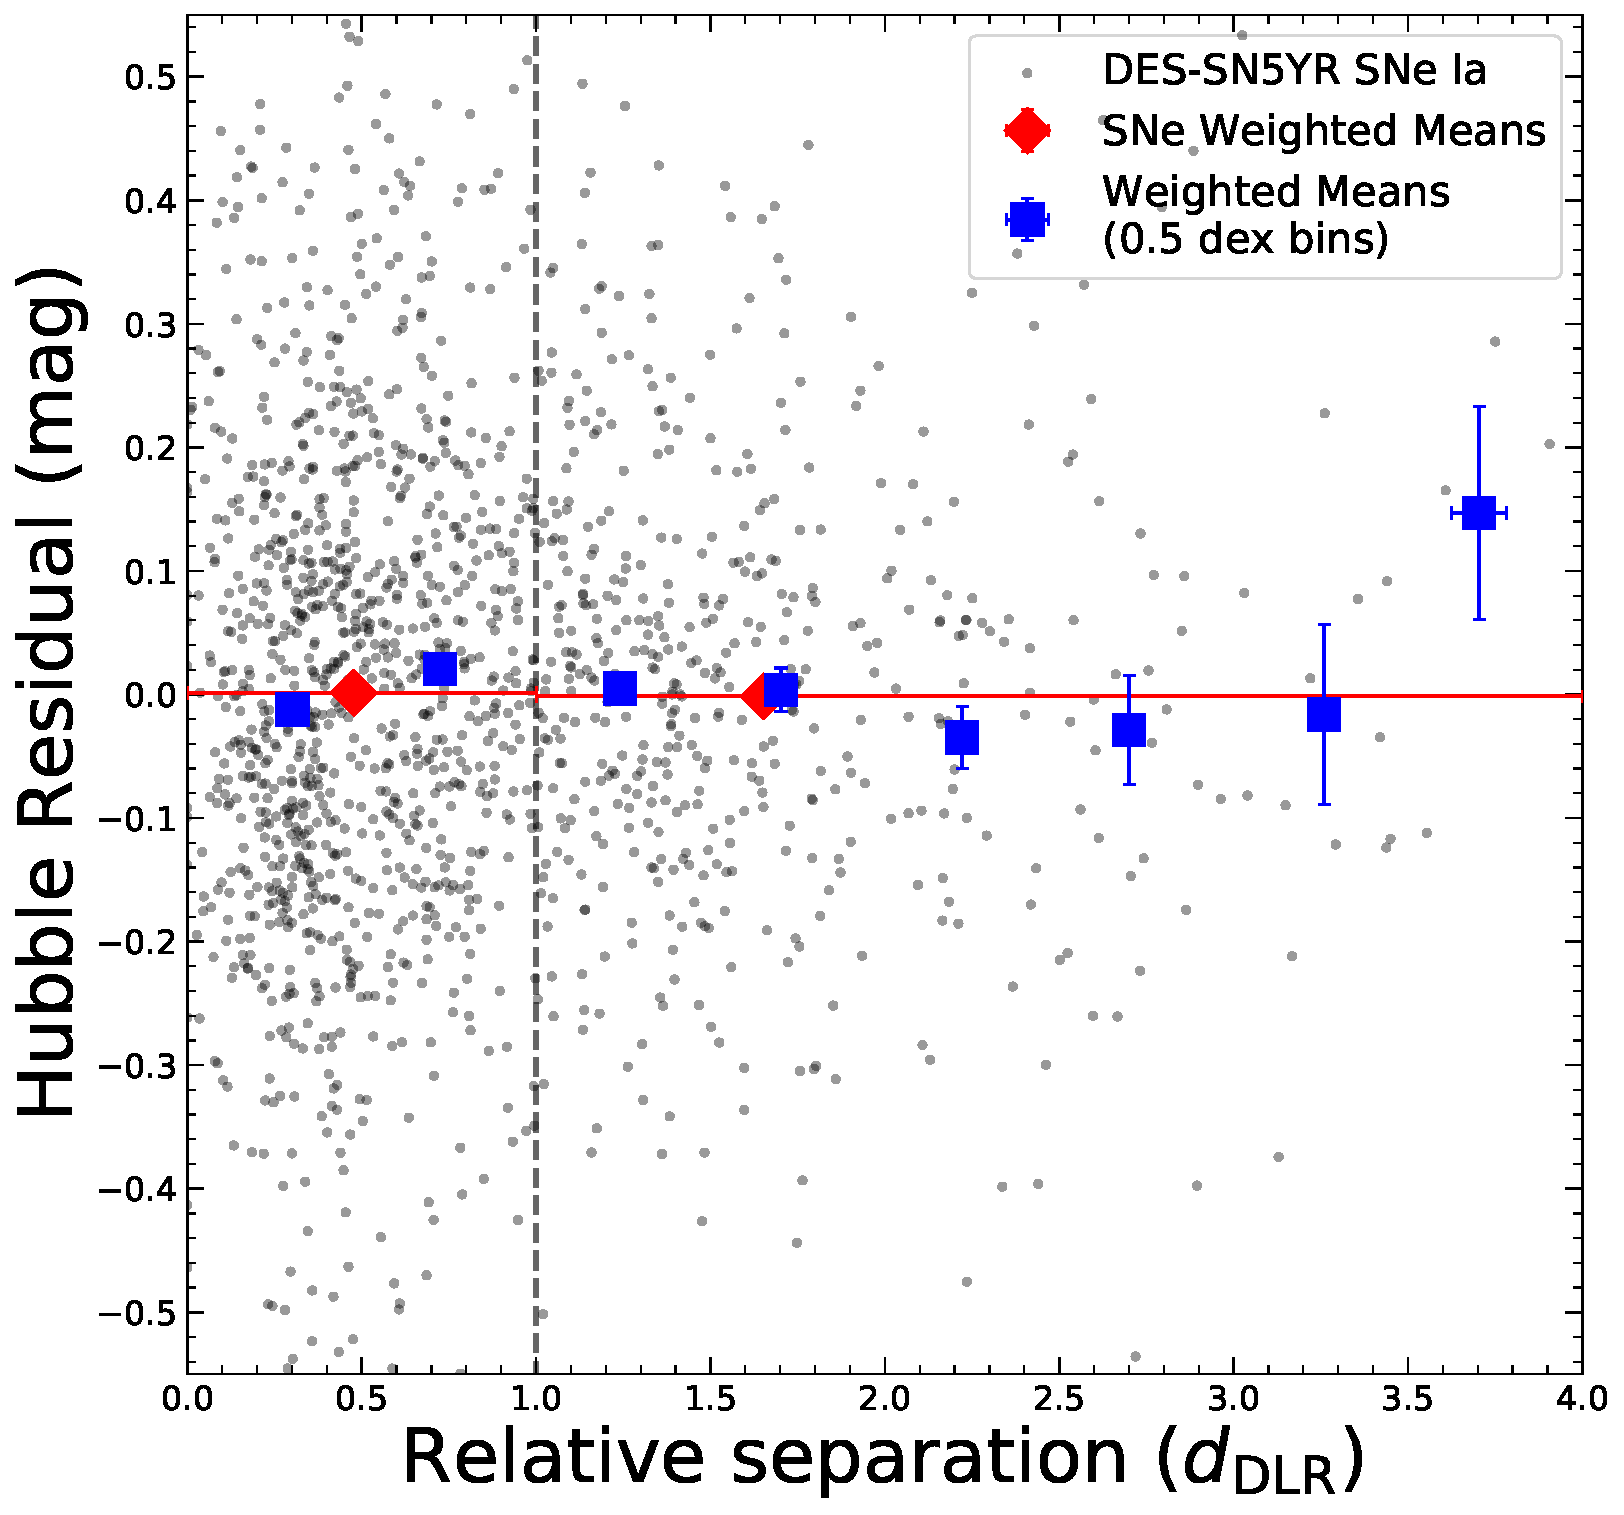
\includegraphics[width=\textwidth]{graphics/Host_galaxy_properties/muresvsddlr.pdf}
         \caption{}
     \end{subfigure}
     
     \vspace{1em} % Adds some vertical space between rows

     % Bottom Two
     \begin{subfigure}[b]{0.45\textwidth}
         \centering
         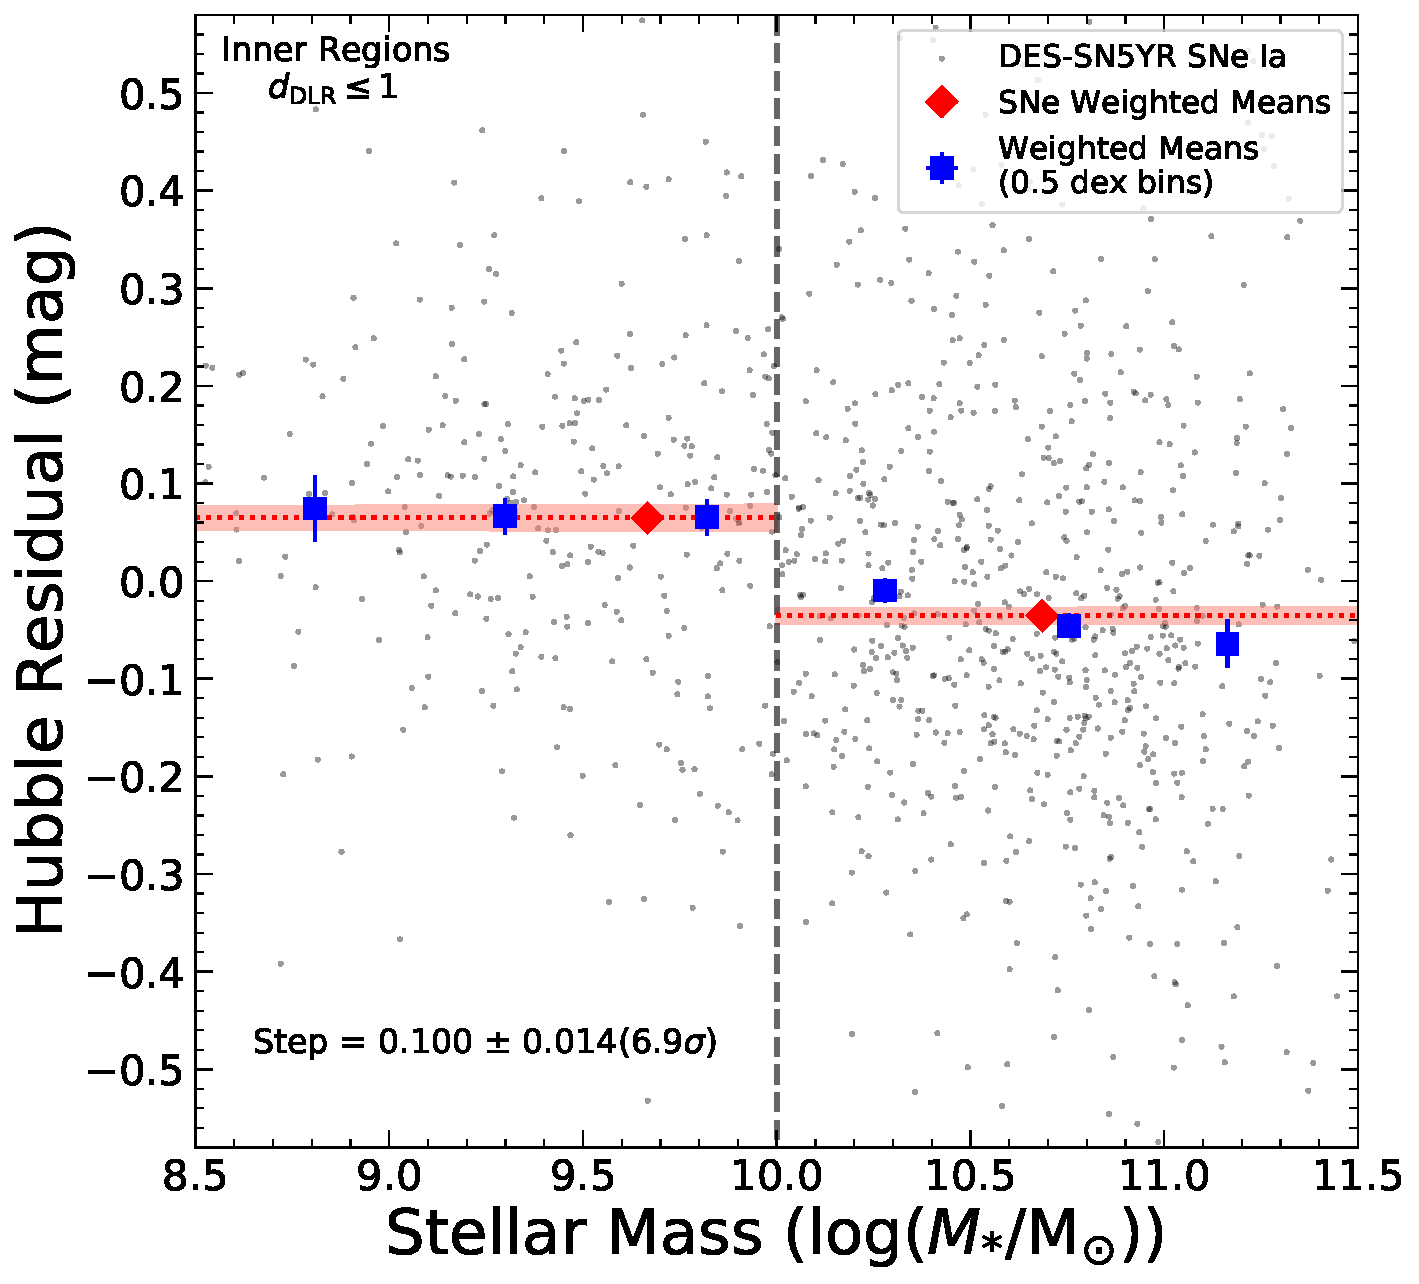
\includegraphics[width=\textwidth]{graphics/Host_galaxy_properties/innerregionsphilsample_extra_binshost_mass_step.pdf}
         \caption{}
     \end{subfigure}
     \hfill
     \begin{subfigure}[b]{0.45\textwidth}
         \centering
         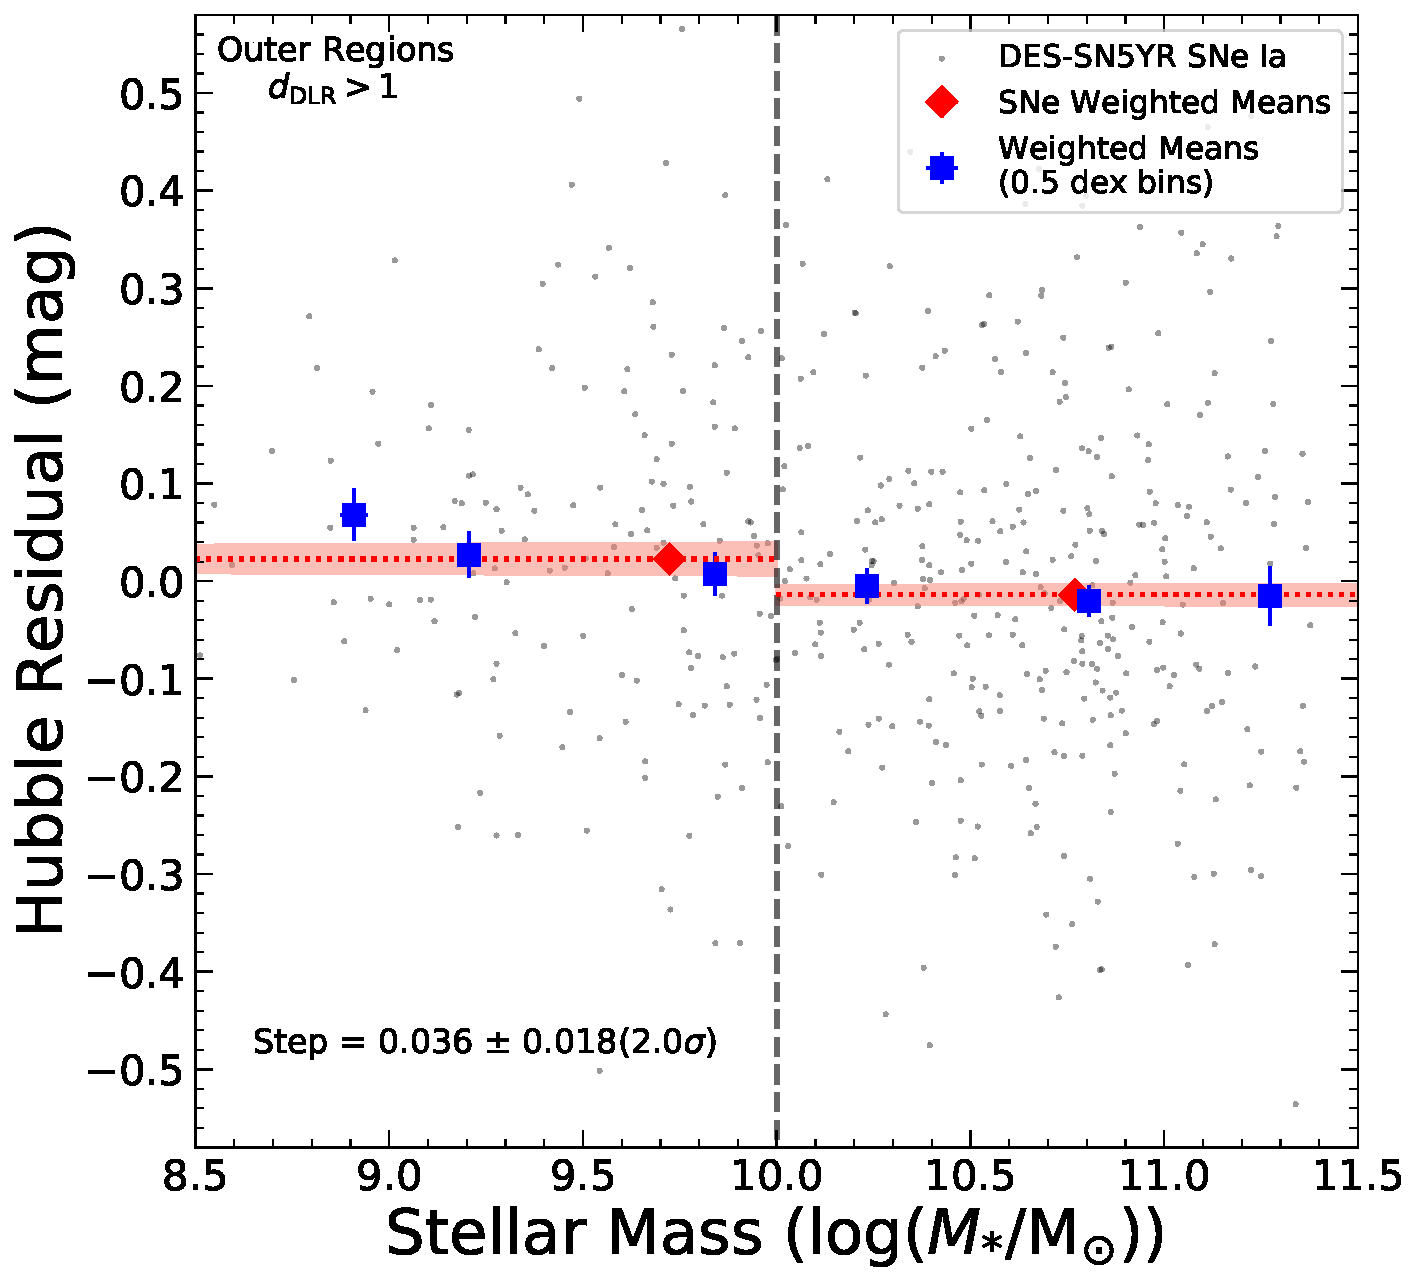
\includegraphics[width=\textwidth]{graphics/Host_galaxy_properties/outerregionsphilsample_extra_binshost_mass_step.pdf}
         \caption{}
     \end{subfigure}
     \caption{Taken from \textcite{toy_reduction_2025}, Figure (a) shows the mass step that can be seen in Figure \ref{fig: Martin et al., 2024 Hubble Residuals as a function of galaxy stellar mass} but as a function of the relative separation from the galaxy centre to the location of the SNe Ia. As a function of the relative separation, it's obvious that the step between Hubble residuals is greatly reduced. In images (b) and (c) which show the Hubble residuals for the inner regions and outer regions respectively, the mass step is found to be reduced for the SNe Ia in the outer regions of their host galaxies.}
     \label{fig: Figures of the mass step being reduced globally but being present within certain regions of the host, from the Marcus Toy paper.}
\end{figure}

By searching for these correlations with the host galaxy properties, an intrinsic property of the SNe Ia's environment could explain this observation of SNe Ia in higher mass galaxies being brighter than those in lower mass galaxies. As seen in \textcite{toy_reduction_2025}, the outer regions of the host galaxy appear to be less affected by whatever is changing the observed brightness of these SNe Ia. 

Another interesting property to study is the global colour of the Host galaxy, \textcite{kelsey_concerning_2022} finds that blue SNe Ia have higher homogeneity in the Hubble residuals. This higher homogeneity in blue SNe Ia was found across the global host galaxy mass, local host galaxy mass, global host galaxy colour and local host galaxy colour. \textcite{kelsey_concerning_2022} interprets this stronger homogeneity post-standardisation as a sign that the older, more globally red galaxies have had more time for SNe to occur and create dust that reddens the SNe Ia that happen afterwards, meaning that the red population is a heterogeneous one and could be made up of a different sub type of SNe Ia that needs to be standardised in a different way to reduce the step function in the residuals.

Another study, \textcite{ramaiya_dependence_2025}, finds correlations with SNe Ia and the stage of evolution that the host galaxy of the SNe Ia. \textcite{ramaiya_dependence_2025} uses 1685 SNe Ia from the DES SN sample and for the host galaxies \textcite{ramaiya_dependence_2025} uses a wide range of sources which include the Canada-France-Hawaii Telescope, the VLT Survey Telescope, the Subaru Hyper Suprime-Cam, the Visible and Infrared Survey Telescope for Astronomy and the Spitzer Space Telescope and the Herschel Space Observatory. This number of sources lets \textcite{ramaiya_dependence_2025} cover a wide range of light emitted from host galaxies for a robust study. As can be seen in Figure \ref{fig: Figure 8 from the Ramaiya et al., 2025 study showing the different colour corrections based on host galaxy stage of evolution.}, the colour nuisance parameter \(\beta\) changes based on the stage of evolution that the host galaxy is in. \textcite{ramaiya_dependence_2025} shows that the stage of the host galaxy's evolution which changes properties such as mass and SFR also affects the luminosities of the SNe Ia in their host galaxies.  

\begin{figure}[htbp]
    \centering
    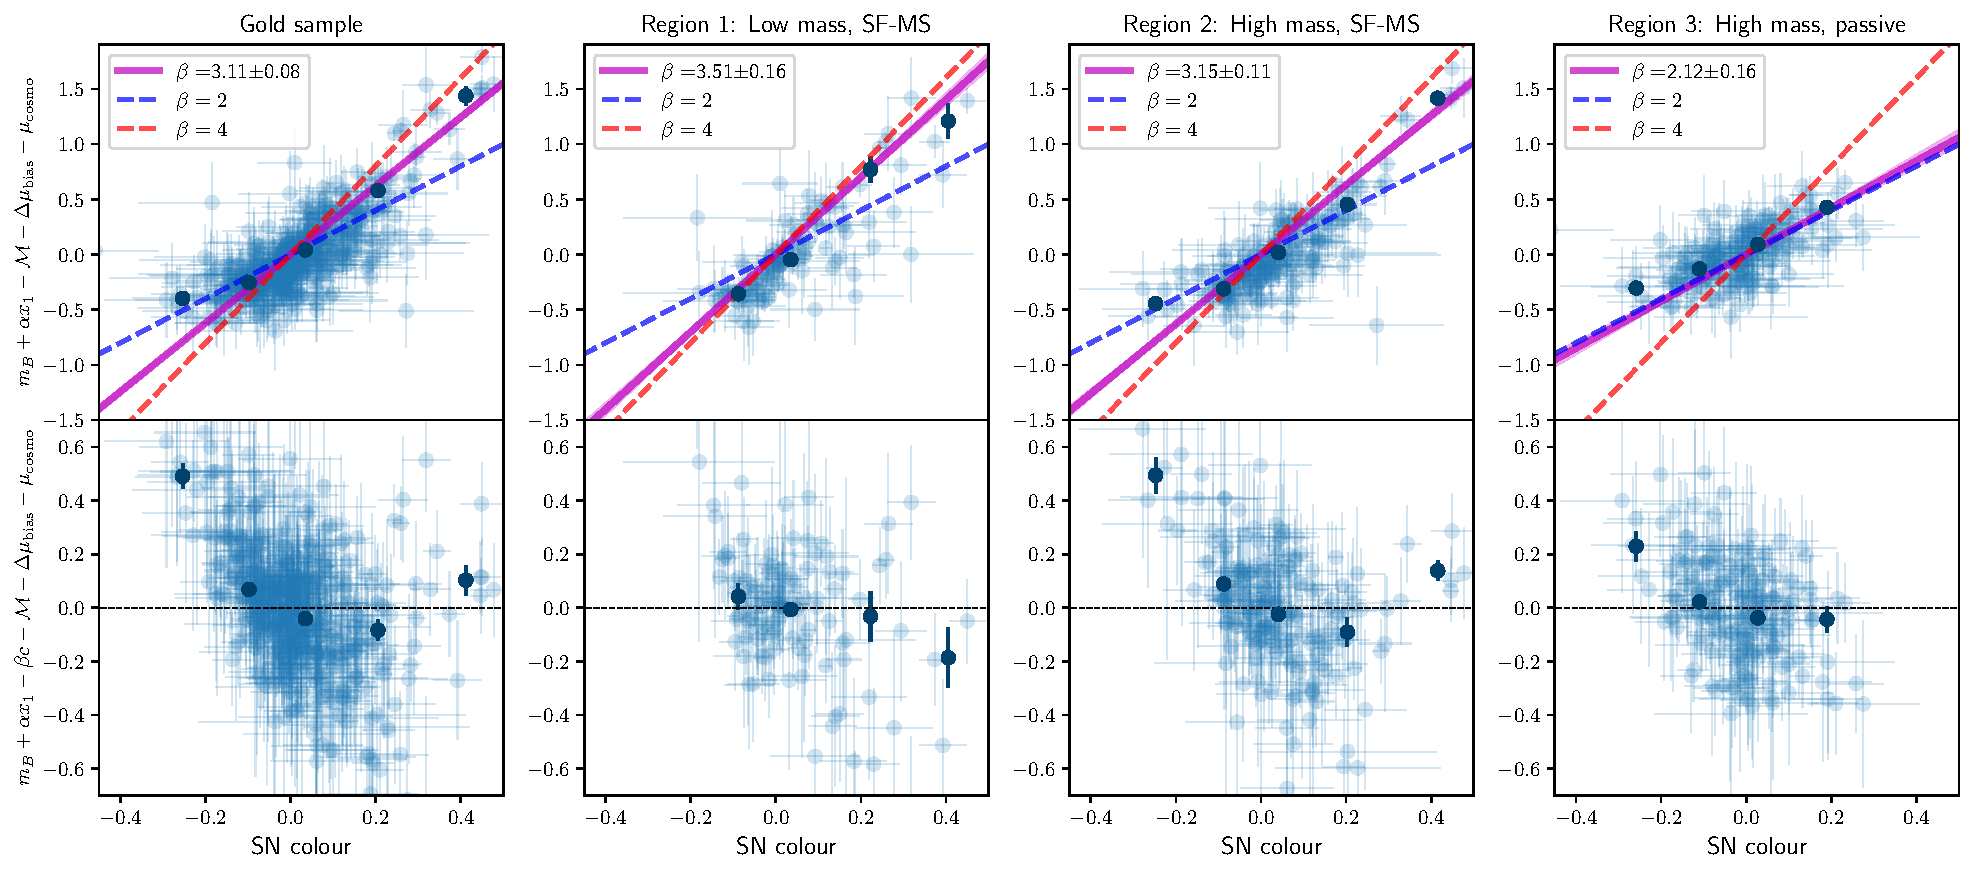
\includegraphics[width=\linewidth]{graphics/Host_galaxy_properties/betas_PLOT.pdf}
    \caption{Taken from \textcite{ramaiya_dependence_2025}, the plots on top are the Hubble residuals plotted as a function of SNe Ia colour, without the colour calibration term in the Tripp equation. The bottom plots show the Hubble residuals whilst correcting for colour as a function of the SNe Ia colour. The gold sample is the sample of all the SNe Ia from the DES SN sample, whilst the remaining three are the plots of the gold sample divided by the evolutionary stage the host galaxy is in.}
    \label{fig: Figure 8 from the Ramaiya et al., 2025 study showing the different colour corrections based on host galaxy stage of evolution.}
\end{figure}

Connecting both \textcite{ramaiya_dependence_2025} and \textcite{kelsey_concerning_2022} shows that the evolutionary stage of the host galaxy and ergo the age has an effect on the magnitudes of the SNe Ia. In \textcite{ramaiya_dependence_2025} \(\beta\) is noticeably different to the active star forming galaxies but once star formation ceases, the colour correction isn't as aggressive. \textcite{kelsey_concerning_2022} finds that hosts with a higher \(U - R\), which is a proxy for a younger star forming galaxy, finds that SNe Ia require a higher \(\beta\) which is also found in \textcite{ramaiya_dependence_2025}. The same relation for more blue galaxies, where \(U - R\) is lower requires smaller \(\beta\). This corroboration of an age-mass relation of host galaxies in \textcite{ramaiya_dependence_2025} and \textcite{kelsey_concerning_2022} shows that the age and evolutionary stage of the host must relate to the SNe Ia in a way that can reduce the scatter in the Hubble residuals.

\subsection{The Environment and Early Excess Flux} \label{subsec: The Environment and Early Excess Flux}
Host galaxy correlations are clearly important in the study of SNe Ia, as understanding the environment where SNe Ia are occurring in can help explain the physics of the SN. The correlations with host galaxy mass, DLR, colour and SFR have helped navigate what could be causing the remaining scatter in the Hubble residuals. But what correlations with host galaxy properties are there for EEx SNe Ia and could they help explain the additional bump in the light curve?   

Due to how small the samples sizes are for EEx SNe Ia, the studies of host galaxy properties correlating with properties of the EEx SNe Ia are limited. \textcite{deckers_constraining_2022} found, whilst acknowledging the small sample size doesn't allow them to make significant conclusions, that 5 of the 6 EEx SNe Ia have hosts with stellar masses lower then the mean of their sample \(<\log(\textup{M}_*/\textup{M}_{\odot})=9.82\). Because of the connection to lower mass hosts, \textcite{deckers_constraining_2022} postulates, stemming from \textcite{rigault_strong_2020} that the progenitor systems of EEx flux SNe Ia are likely to be from a younger population. 

A recent study by \textcite{wu_wfst_2026} uses a sample of 16 SNe Ia with data 16 days before the B band maximum light. \textcite{wu_wfst_2026} found 3 EEx Flux SNe Ia and could only associate two with a host galaxy, the conclusions are limited due to the limited data, regardless both the associated hosts of the 2 EEx SNe Ia had a lower stellar mass than the mean of the sample (\(\log(\textup{M}_*/\textup{M}_{\odot})=9.94\)). Whereas only one of the SNe Ia occurred in a host with a highest SFR of the sample (3.64\(\textup{M}_{\odot}yr^{-1}\)) whereas the second SNe Ia has the 4 lowest SFR of the sample. 

It is safe to say that without more detections of EEx SNe Ia, correlations with host galaxy properties will not be able to reach a sample size that allows for statistically significant analysis. This results in a lack of conclusions being able to be drawn about the niche phenomena observed in these light curves.